\pdfminorversion=4
\documentclass{beamer}
\usetheme{default}
\usepackage{epsfig}
\usepackage{pstricks,pst-coil}
\usepackage[spanish]{babel}
\usepackage[utf8]{inputenc}


\newcommand{\pp}{$pp$}
\newcommand{\ppb}{$p$+Pb}
\newcommand{\dau}{$d$+Au}
\newcommand{\aau}{Au+Au}
\newcommand{\snn}{\sqrt{s_{_{NN}}}}
\newcommand{\gev}{GeV/$c$}
\newcommand{\pt}{p_{T}}
\newcommand{\dphi}{\Delta\phi}
\newcommand{\deta}{\Delta\eta}
\newcommand{\bd}[1]{{\bf #1}}
\newcommand{\g}[1]{\vec{g}_{#1}}

\title[ML PID]
{Identificación de partículas en el experimento NICA utilizando técnicas de inteligencia artificial de análisis multivariante}

\author[Dra. Isabel Domínguez Jiménez]
{Dra. Isabel Domínguez Jiménez \\
Facultad de Ciencias Físico-Matemáticas \\
Universidad Autónoma de Sinaloa }

\institute[FCFM-UAS]
{~}


\date[]
{\today}

\AtBeginSubsection[]
{
  \begin{frame}<beamer>
    \frametitle{}
    \tableofcontents[currentsection,currentsubsection]
  \end{frame}
}

\begin{document}

\begin{frame}
  \titlepage
\end{frame}


%%%%%%%%%%%%%%%%%%%%%%%%%%%%%%%%%%%%%%%%%%%%%%%%%%%%%%%%%%%%%%55
\begin{frame}{Piones}
\textit{Regresión Logística: auc=1.000 f1=1.000 }

\begin{center}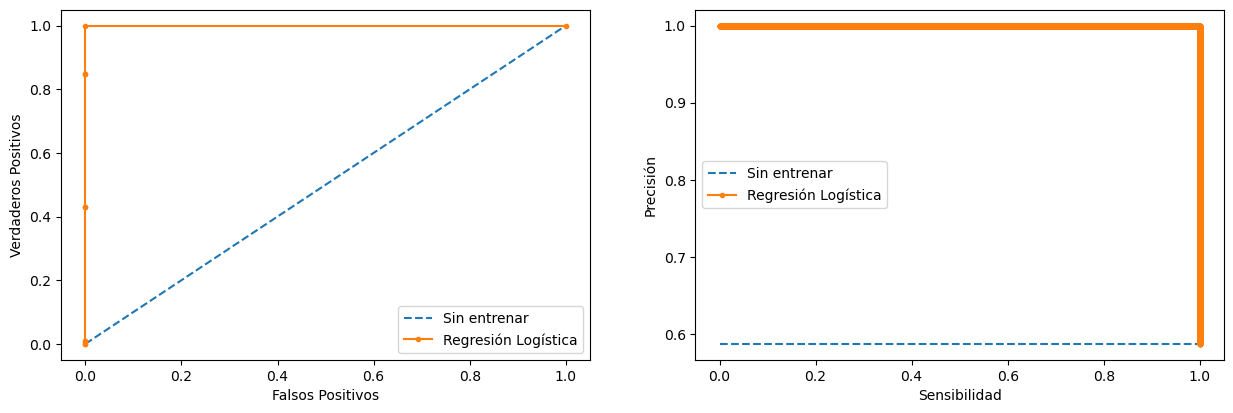
\includegraphics[scale=0.35]{figure/pi.png}\end{center}

\end{frame}
%%%%%%%%%%%%%%%%%%%%%%%%%%%%%%%%%%%%%%%%%%%%%%%%%%%%%%%%%%%%%%55
\begin{frame}{Protones}
	\textit{Regresión Logística: auc=0.941 f1=0.874}
	
	\begin{center}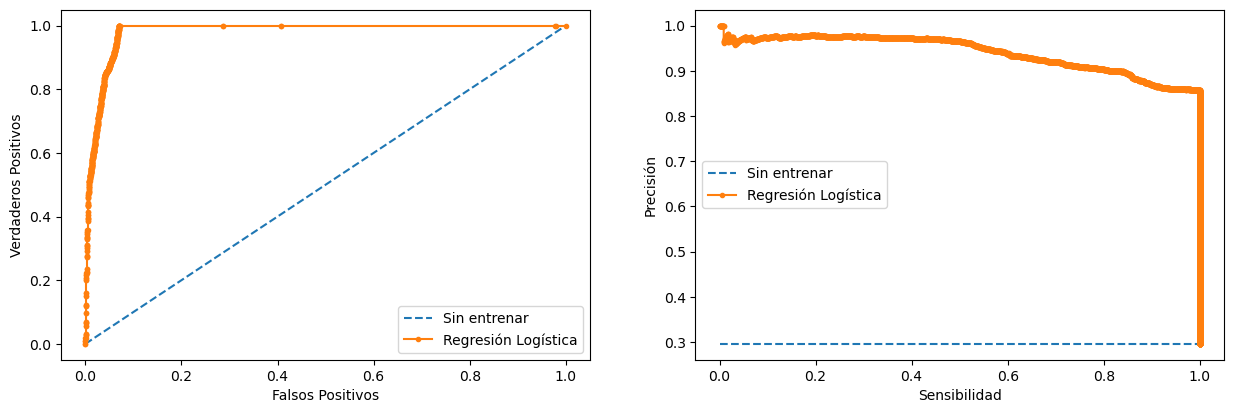
\includegraphics[scale=0.35]{figure/p.png}\end{center}

\end{frame}
%%%%%%%%%%%%%%%%%%%%%%%%%%%%%%%%%%%%%%%%%%%%%%%%%%%%%%%%%%%%%%55
\begin{frame}{Kaones}
	\textit{Regresión Logística: auc=0.042 f1=0.000}
	
	\begin{center}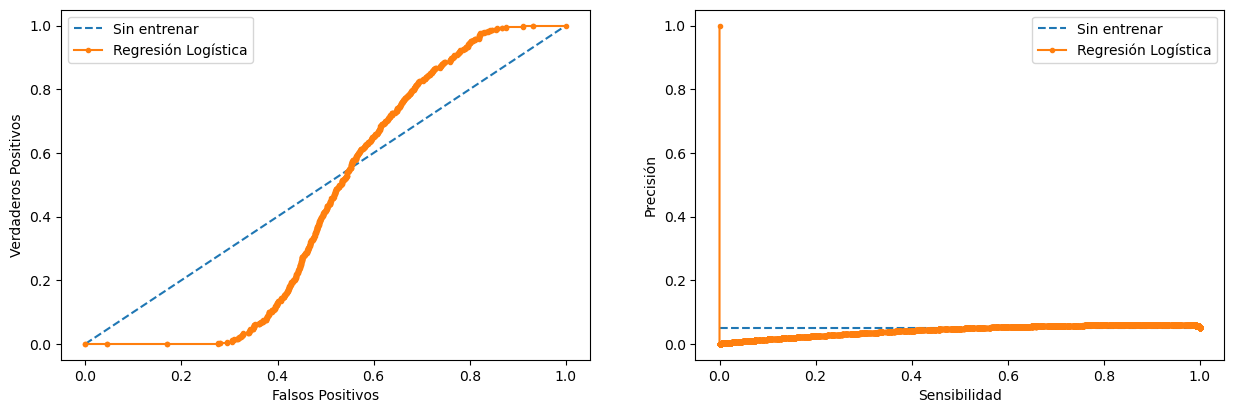
\includegraphics[scale=0.35]{figure/k.png}\end{center}
	
\end{frame}
%%%%%%%%%%%%%%%%%%%%%%%%%%%%%%%%%%%%%%%%%%%%%%%%%%%%%%%%%%%%%%55
\begin{frame}{Lambda}
	\textit{Regresión Logística: auc=0.007 f1=0.000 }
	
	\begin{center}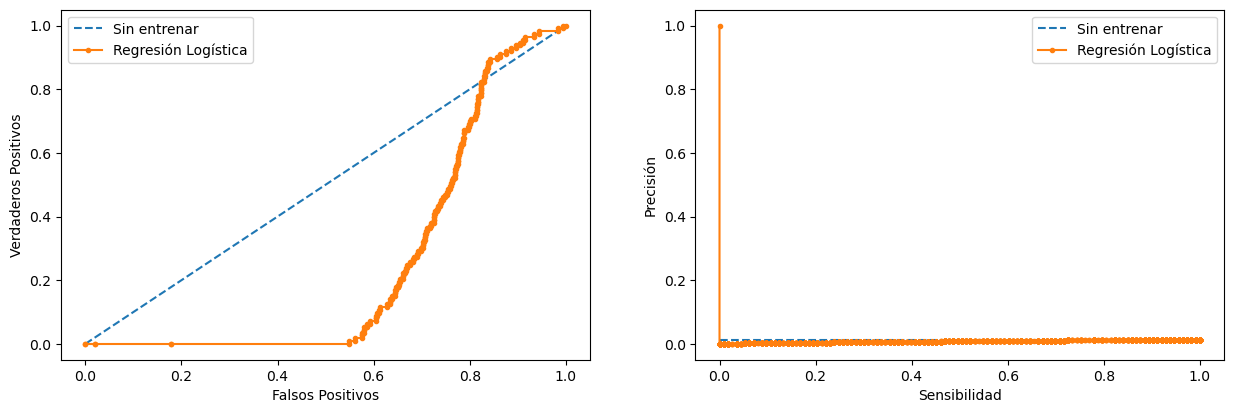
\includegraphics[scale=0.35]{figure/lambda.png}\end{center}
	
\end{frame}

\end{document}
